%\documentclass{amsart}

\documentclass{article}
\usepackage[letterpaper,hmargin=0.8in,vmargin=0.8in]{geometry}
\usepackage[nosetup, colorlinks]{tony}
\usepackage{graphicx}

\usepackage{amsmath,amssymb}
\usepackage{siunitx}

\usepackage{mathpazo}
\usepackage{microtype}
\usepackage{multicol}

\usepackage{diagbox}

\usepackage{color}
\usepackage[dvipsnames]{xcolor}
%\usepackage[printwatermark]{xwatermark}
%\newwatermark*[allpages,color=gray!50,angle=45,scale=3,xpos=0,ypos=0]{DRAFT}

\usepackage{tikz}
\usetikzlibrary{arrows}
\usetikzlibrary{angles,patterns,calc}

\DeclareMathOperator{\sgn}{sgn}
\DeclareMathOperator{\NLL}{NLL}
\newcommand{\sind}[1]{^{(#1)}}

\newcommand\halfwidth{3.25in}

\title{Prediction of airline departure delays}
\author{Tony Zhang and Menghua Wu}
\date{December 16, 2016}

\begin{document}
\maketitle

\begin{multicols}{2}

% % % % % % % % % %
%    INTRODUCTION
% % % % % % % % % %

\section{Introduction}

Often, people purchase plane tickets
to minimize monetary cost.
However, price is not the only consideration
when consumers purchase tickets---not
all flights are created equal.
In particular,
flyers often care about and take into account
the risk that a flight will be delayed.
This paper hopes to quantify this risk
on the basis of past flight delay data.

The United States Bureau of Transportation Statistics (BTS)
compiles comprehensive datasets annually
regarding the nation's transportation infrastructure,
including aviation, maritime, highway, and rail.~\cite{bts}
In this paper, we focus on the aviation dataset,
which reports on a wide range of variables concerning individual flights,
including carrier, origin and destination, and flight delays.
We will primarily concern ourselves with classification:
whether a flight is delayed or not.

% TODO change this section?
We downloaded data from the month of June 2015,
with a total of approximately 500000 individual flights.
Notably, some of the data is missing.
We used these data to build a classifier
that predicts whether or not a flight's departure
is expected to be delayed.
We applied several methods of classification
and compare their results here.

While we will briefly remind the reader
of particular aspects of each model,
we assume familiarity them.
As a reference for implementation details and model specifics,
we direct the reader to \cite{sklearn-ug}.

\section{Data preprocessing}

For simplicity,
we only considered the following data features:
\begin{itemize}
    \item
    Departure date and time
    \item
    Airline
    \item
    Origin and destination airports
\end{itemize}

Since airline and airports are categorical features,
we encoded them as one-hot vectors.
In the data subset we considered,
there were 14 airlines and roughly 250 airports.

For date and time,
we began by encoding them as days into a year
and minutes into the day.
This representation leaves much to be desired, however.


\subsection{Cyclic features}
\label{subsec:cyc-feat}

Features such as time of day and day of year
are naturally cyclic.
Representing them on a linear scale
therefore imposes an unnatural metric on them.
For instance,
if we naively represent times as ``minutes into day",
the time 23:59 will be considered ``more similar"
by any machine learning model to noon than to 00:01,
which disagrees with our intuitive notions of closeness.

A better representation of cyclic data
would respects our notions of closeness.
An obvious choice is to map a linear data point $x \in [0, T)$
onto a unit circle by
\begin{equation}
    \label{eq:cyc-mapping}
    x \mapsto \lt(\cos\f{2\pi x}{T}, \sin\f{2\pi x}{T}\rt).
\end{equation}
For instance, if we were to encode the time of day,
noon would have ``angle" $\f{2\pi x}{T} = \pi$
and would thus get mapped to the point $(-1, 0)$:

\begin{center}
    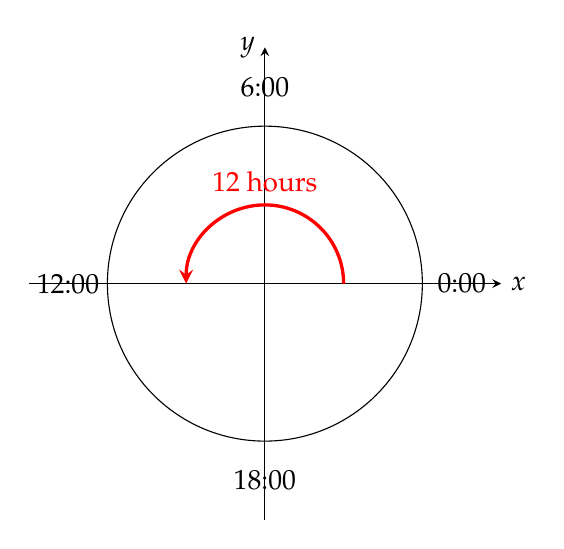
\begin{tikzpicture}
  \tikzset{>=stealth}
  % draw axises and labels. We store a single coordinate to have the
  % direction of the x axis
  \draw[->] (-3,0) -- ++(6,0) coordinate (X) node[right] {$x$};
  \draw[->] (0,-3) -- ++(0,6) node[left] {$y$};

  \newcommand\CircleRadius{2cm}
  \newcommand\TextRadius{2.5cm}
  \draw (0,0) circle (\CircleRadius);
  
  \node at (0:\TextRadius) {0:00};
  \node at (90:\TextRadius) {6:00};
  \node at (180:\TextRadius) {12:00};
  \node at (270:\TextRadius) {18:00};
  
  \draw
  (0,0) 
  coordinate (O) % store origin
  -- 
  (180:\TextRadius)
  coordinate (P)
  -- 
  (P |- O) coordinate (Px)
  
  % pic trick is from the angles library, requires the three points of
  % the marked angle to be named
  pic [draw,red,very thick,->,angle radius=1cm,pic text=12 hours,
  angle eccentricity=1.3] {angle=X--O--P};

\end{tikzpicture}
\end{center}

We encoded dates (with $T$ being a year)
and time (with $T$ being a single day)
in this fashion.
In preliminary testing,
we found that this encoding
noticeably improved classification accuracies
for a variety of models,
including logistic regression and random forests.

\subsection{Dataset partitioning}

For the purposes of the following experiments,
we limited ourselves to a random sample of 40000 flights
from June 2015;
we found this size a good compromise between computational tractability
and sample representativeness.
We partitioned the data points into training, validation, and test sets,
with $80/10/10\%$ of the data, respectively.


\section{Logistic regression}
\label{sec:logreg}

To establish a baseline accuracy
and to benchmark our future efforts,
we began with a standard implementation
of a logistic regression classifier
with $L_2$ regularization.
Recall that such a classifier attempts to minimize a loss of the form
\begin{equation}
    \label{eq:log-reg-l2-loss}
    J(w, b) = \f12 w^T w + C \sum_i \log\lt(1 + e^{-y\sind{i}(w^T x\sind{i} + b)}\rt)
\end{equation}
where the sum is taken over all training data points.
The parameter $C$ controls the amount of regularization;
a smaller value of $C$ produces greater regularization.

We performed a sweep over log-uniformly spaced $C$
from $10^{-5}$ to $10^5$ (with factors of 10 between each $C$).
Optimizing for validation accuracy,
we selected $C^* = 100$,
which yielded a test accuracy of $0.661$.

Unsurprisingly,
replacing the first term in Equation~\ref{eq:log-reg-l2-loss}
with an $L_1$ norm on $w$
gives us the loss function for a classifier with $L_1$ regularization.
Performing a sweep over $C$ as we did previously
and optimizing for validation accuracy again,
we found an almost identical test accuracy of $0.660$.

We present the validation accuracies
under both regularization schemes
for the values of $C$ we tested
in Figure~\ref{fig:log-reg-c-sweep}.

\begin{figure*}[t] %  figure placement: here, top, bottom, or page
   \centering
   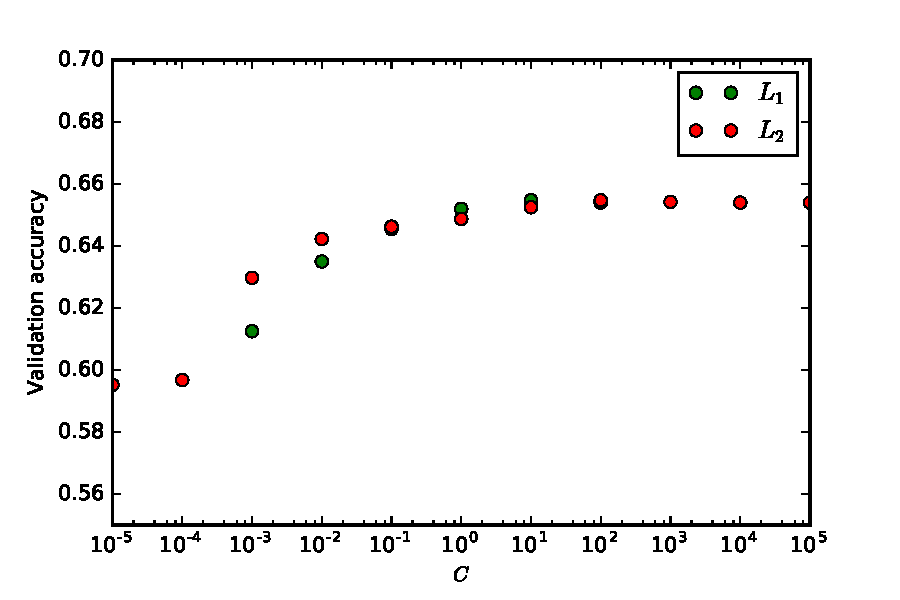
\includegraphics[width=4.5in]{img/log-reg-C-sweep.pdf}
   \caption{Logistic regression validation accuracies
   under $L_1$ and $L_2$ regularization
   for varying values of regularization parameter $C$.}
   \label{fig:log-reg-c-sweep}
\end{figure*}


\section{Multilayer perceptrons}

We next attempted to improve upon our previous results
with multilayer perceptrons:
vanilla neural networks.
With an existing implementation,
we minimized mean cross-entropy loss with the Adam optimizer,
computing gradients by backpropagation.
Recall that cross-entropy loss for a single data point $x\sind{i}, y\sind{i}$
is given by
\begin{equation}
    J\sind{i}(w) = -y\sind{i}\log\hat y\sind{i} - (1-y\sind{i})\log(1-\hat y\sind{i})
\end{equation}
where $y\sind{i}$ is a binary training label (either 0 or 1)
and where $\hat y\sind{i}$ is the probability estimate from the network.

We also imposed $L_2$ regularization on the network weights,
governed by regularization parameter $\alpha$,
such that the training loss function is given by
\begin{equation}
    J(w) = \f12\alpha w^T w + \sum_i J\sind{i}(w).
\end{equation}

We experimented with various architectures, activations, and $\alpha$.
Given the large space of possible hyperparameter combinations,
it was infeasible to find a best set of hyperparameters exhaustively.
As such,
we explored the effects of each hyperparameter
by holding values of the others fixed.

\subsection{Architecture}

In experimenting with network architecture,
we fixed $\alpha = 10^{-5}$.
We began by exploring different numbers of hidden layers,
finding that deeper networks provided no significant improvement
over single-hidden-layer networks.
Thus, we restricted our attention
to networks with just a single hidden layer.

We show our findings in Figure~\ref{fig:mlp-plots}
for three different activation functions on the hidden nodes;
it's apparent that varying the number of hidden nodes
did not provide any substantive improvement in our results
over our baseline.

\begin{figure*}[t] %  figure placement: here, top, bottom, or page
   \centering
   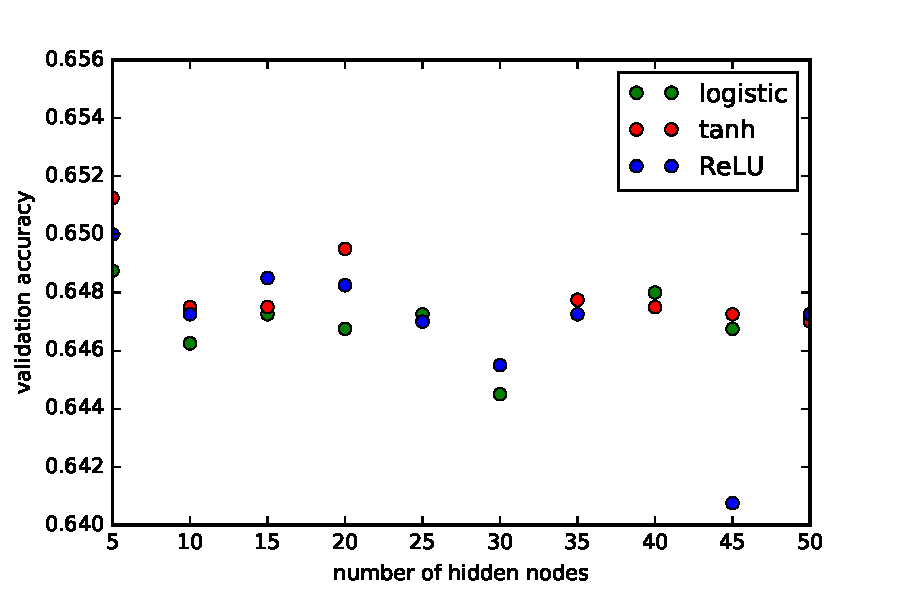
\includegraphics[width=\halfwidth]{img/mlp-one-hidden-layer.pdf}
   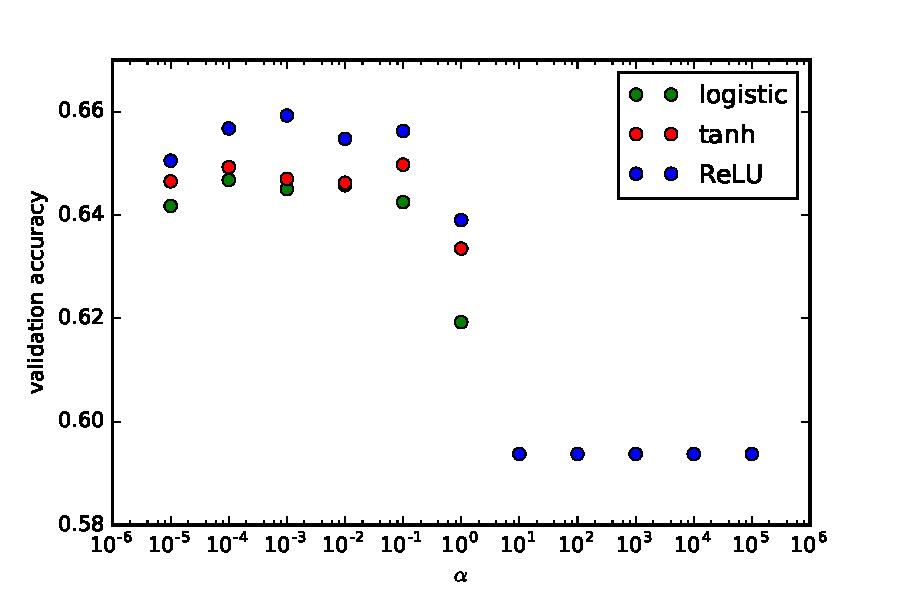
\includegraphics[width=\halfwidth]{img/mlp-alpha-experiment.pdf}
   \caption{Single-layer multilayer perceptron validation accuracies.
   The plot on the left shows the results of varying the number of hidden nodes
   while fixing $\alpha = 10^{-5}$.
   On the right, we fixed the size of the hidden layer at 25 nodes
   and varied $\alpha$.}
   \label{fig:mlp-plots}
\end{figure*}


\subsection{Regularization}

To see the effects of regularization,
we considered networks with logistic, tanh, and ReLU activations
on a single hidden layer of 25 nodes.
As we did for the parameter $C$ in section~\ref{sec:logreg},
we performed a sweep over log-uniformly spaced $\alpha$ from $10^{-5}$ to $10^5$.
We present our results in Figure~\ref{fig:mlp-plots}.
We see marginally better performance by the ReLU model with $\alpha=10^{-3}$.
With a test accuracy of $0.647$, however,
this model did not improve upon our logistic regression baseline.


\section{Random forest classification}

We next turned to ensemble methods
to improve upon our previous results.
We began by experimenting with
existing implementations of random forest classifiers.
In particular,
we explored the effects of varying hyperparameters such as
\begin{itemize}
    \item
    bootstrapping
    \item
    number of decision trees
    \item
    impurity threshold
    \item
    maximum tree depth
    \item
    feature masking
    \item
    warm starting
\end{itemize}

\begin{figure*}[t]
   \centering
   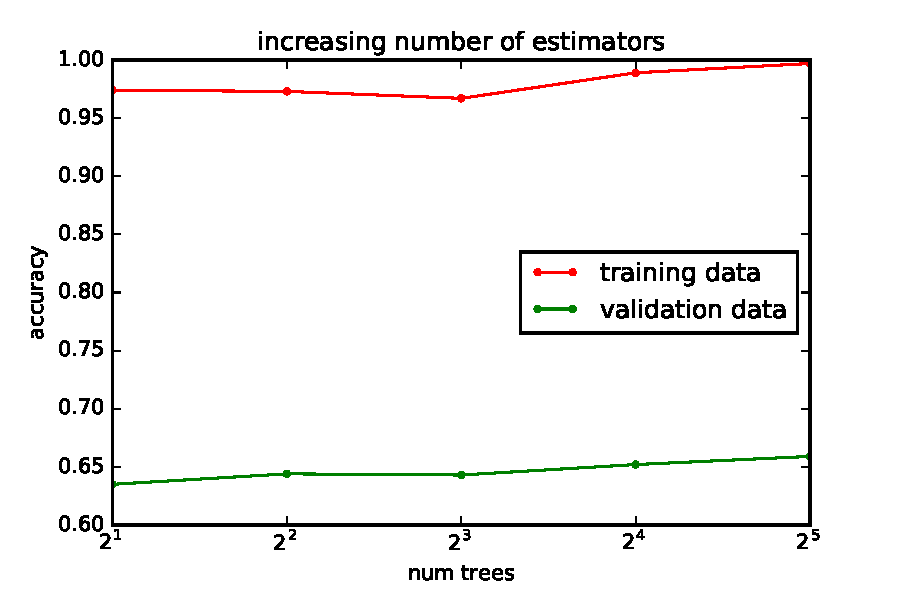
\includegraphics[width=\halfwidth]{img/rf-numEstimators.pdf}\hspace{-.1in}
   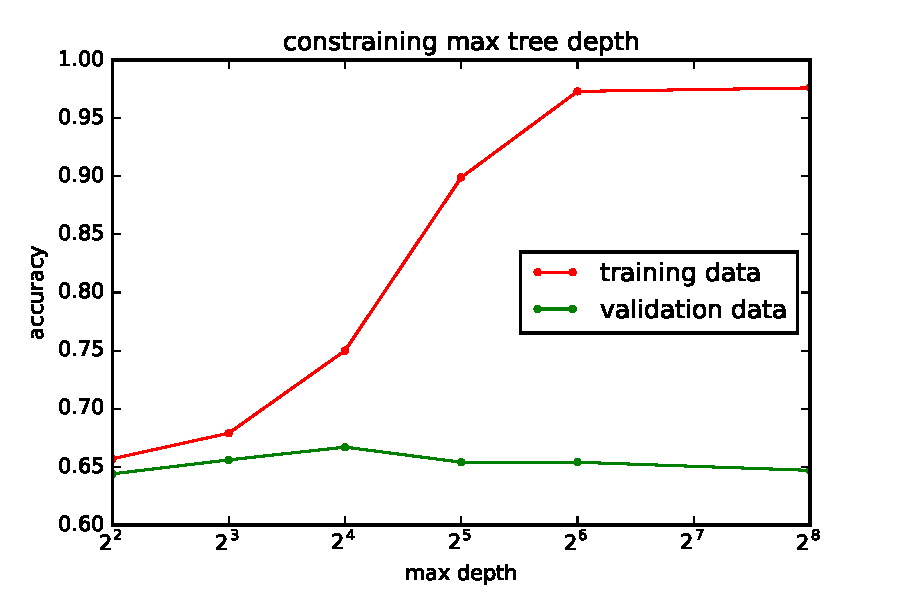
\includegraphics[width=\halfwidth]{img/rf-maxTreeDepth.pdf}
   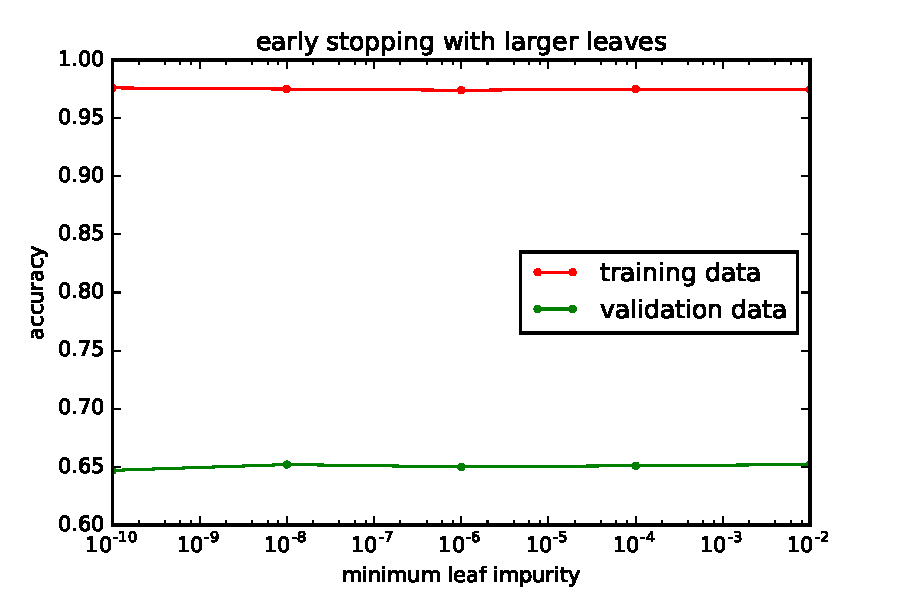
\includegraphics[width=\halfwidth]{img/rf-impurity.pdf}\hspace{-.1in}
   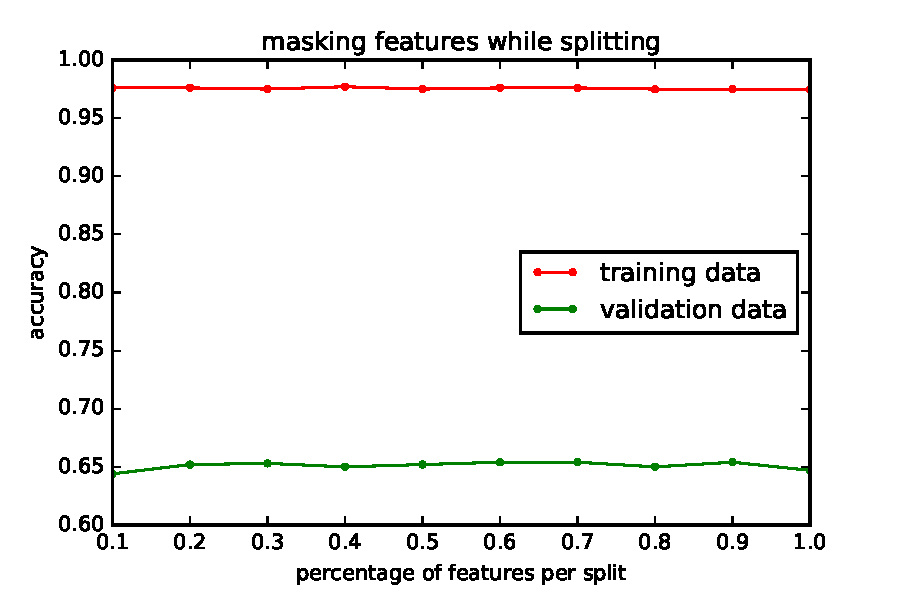
\includegraphics[width=\halfwidth]{img/rf-maskingFeatures.pdf}
   \caption{Varying parameters for random forest classifier.
     Setting a minimum impurity on leaves and feature masking
     do not significantly affect validation or testing accuracy.}
   \label{fig:rf-params}
\end{figure*}

%We leveraged existing random forest implementations
%and determined the optimal parameters for classifying our data.
%We determined the best model using our validation data
%and tested on our testing data.
%There may be strong relationships between
%month of year and airline delay,
%as the holiday season is often associated with
%inclement weather and an increase in delays.
%Therefore, we trained a separate random forest classifier
%for each month, in additional to a single classifier
%for the combined data.
%For each month,
%the resultant model was an average of
%that month's classifier and the combined classifier,
%weighted by validation error.
%On the testing data,
%the combined classifier performed better
%than each classifier alone,
%perhaps due to increased generalization.

In the following sections,
we explore the effects of varying hyperparameters,
by tweaking the value of one at a time,
holding all else equal to the following defaults:
bootstrapped samples,
10 estimators,
a maximum leaf-node impurity threshold of $10^{-7}$,
and no maximum tree depth,
feature masking, or warm start.
Trees were trained under Gini impurity.
The results of these experiments
are presented graphically in Figure~\ref{fig:rf-params}.

\subsection{Bootstrapping}

Recall that bootstrapping involves
training estimators on subsets of the training data
sampled \emph{with} replacement from the dataset,
emulating sampling from the general population.
When we sampled without replacement instead
(i.e. no bootstrapping),
training accuracy increased,
but validation accuracy decreased,
potentially due to overfitting on more sample points during training.

% bootstrap
%Training data score 0.9757875
%Testing data score 0.6527087149960743
%
% no bootstrap
%Training data score 0.9998625
%Testing data score 0.6186862077990055
\begin{center}
    \begin{tabular}{c| c c}
        method & bootstrap & no bootstrap \\\hline
        training acc
        		& 0.976 & 0.999 \\
        validation acc
        		& 0.653 & 0.619
    \end{tabular}
\end{center}

\subsection{Number of estimators}

A key hyperparameter in random forests,
as in all enesemble methods, is the number of estimators,
which impacts overfitting and prediction accuracy.
Increasing the number of trees
improved both training and validation accuracy.
However, since training more estimators
is computationally intensive,
we did not train more than 32 trees.
Our results are as follows and in Figure~\ref{fig:rf-params}.
%n_estimators 2
%Training data score 0.9739375
%Testing data score 0.6351740382098927
%
%n_estimators 8
%Training data score 0.9671375
%Testing data score 0.6430253860246009
%
%n_estimators 16
%Training data score 0.9887
%Testing data score 0.6517927244176916
%
%n_estimators 32
%Training data score 0.9971375
%Testing data score 0.6585972258571055
\begin{center}
    \begin{tabular}{c|c c c c}
        $n$ trees
        		& 2 & 8 & 16 & 32 \\\hline
        training acc
        		& 0.974 & 0.967 & 0.989 & 0.997\\
        validation acc
        		& 0.635 & 0.643 & 0.651 & 0.658
    \end{tabular}
\end{center}

We see that there is slight,
but nontrivial, improvement in validation accuracies
as our ensemble grows.

\subsection{Maximum tree depth}

By default,
the depths of the individual decision trees are unconstrained,
so that the model training runs until all nodes
are expanded into valid leaves.
We experimented with imposing a maximum depth
as a form of early stopping.
Unsurprisingly,
a maximum depth generally decreased training accuracy,
but increased validation accuracy
in some cases.
%max_depth_leaf 4
%Training data score 0.6570625
%Testing data score 0.6447265113844544
%
%max_depth_leaf 8
%Training data score 0.679025
%Testing data score 0.6563726773096048
%
%max_depth_leaf 16
%Training data score 0.75025
%Testing data score 0.6665794294687255
%
%max_depth_leaf 32
%Training data score 0.8992
%Testing data score 0.6656634388903429
%
%max_depth_leaf 64
%Training data score 0.9726625
%Testing data score 0.6540172729651924
%
%max_depth_leaf 256
%Training data score 0.976025
%Testing data score 0.6472127715257786
\begin{center}
    \begin{tabular}{c|ccccc}
        max depth &
          4 & 8 & 16 & 32 & 256 \\\hline
        training acc. &
          0.657 & 0.679 & 0.750 & 0.899 & 0.976\\
        validation acc. &
          0.644 & 0.656 & 0.667 & 0.654 & 0.647
    \end{tabular}
\end{center}
Indeed, a maximum tree depth effectively
reduces overfitting to training data
by regularizing the complexity of individual decision trees.

\subsection{Masking features}

When building each tree,
we can ignore a subset of features
when looking for the best split.
Feature masking did not significantly affect
training or validation accuracy.
This may be due to the sparsity of our data,
a consequence of our use of one-hot encodings.

\subsection{Early stopping}

If we do not constrain the depth of the tree,
an alternative regularization appraoch
is to increase the minimum tolerable Gini impurity at each leaf.
However,
changing this value had little effect,
and was not as effective as limiting tree depth.

\subsection{Warm start}

For each estimator,
we can either train a new tree from scratch (default),
or use the results of the previous run
as a starting point (warm start).
Preliminary experiments showed that using a warm start
had little effect.
We did not explore usage of warm starts further.

\subsection{Optimal model}

Based on validation accuracy,
we selected the best model
of 32 estimators, a max depth of 16,
and default values for all other parameters.
We obtained a testing accuracy of 0.687,
a slight, but significant, improvement
on our logistic regression baseline.

\section{Boosting}

We tried various boosting methods using existing libraries
and tested different weak learners as the base estimator,
which we discuss below.

\subsection{Adaboost-SAMME}

We also applied a variant of the Adaboost algorithm,
Adaboost-SAMME (stagewise additive modeling
with a multi-class exponential loss function).

\begin{figure*}[t]
   \centering
   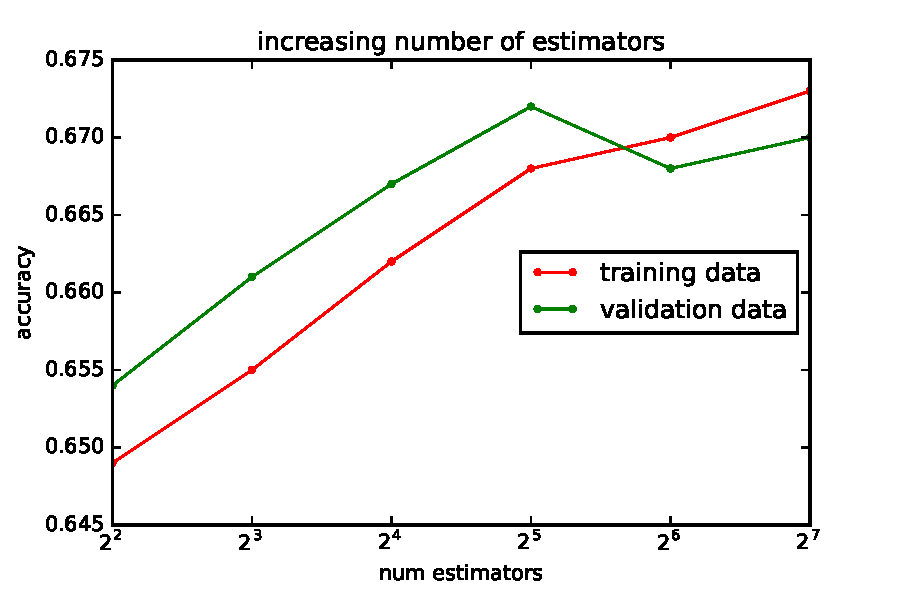
\includegraphics[width=\halfwidth]{img/adaB-numEstimators.pdf}\hspace{-.1in}
   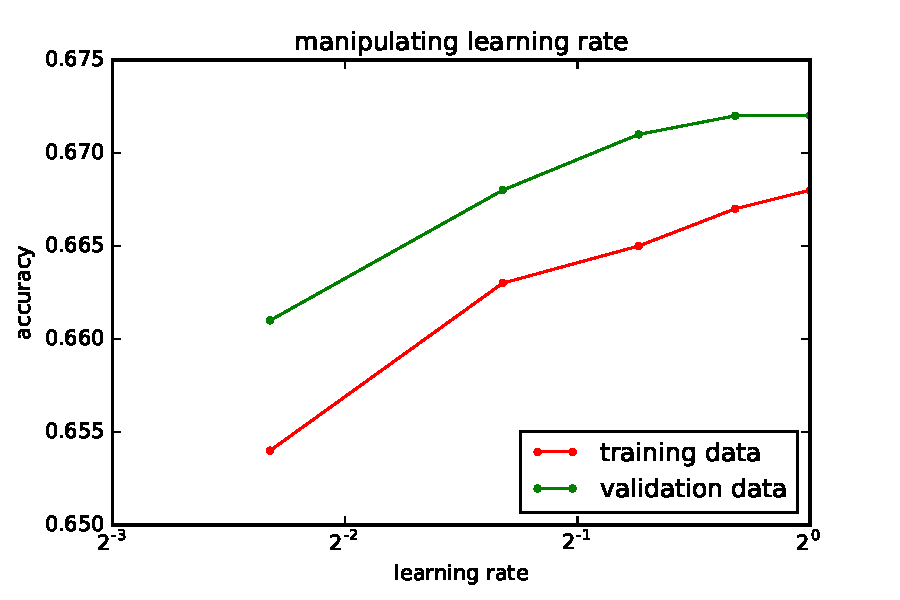
\includegraphics[width=\halfwidth]{img/adaB-learningRate.pdf}
   \caption{Varying parameters for the Adaboost-SAMME classifier,
   with a decision tree weak learner.
   Increasing number of estimators accuracy,
   but decreasing learning rate did not improve results.
   }
   \label{fig:adaB-params}
\end{figure*}

With an ensemble of 50 decision tree classifiers,
the Adaboost algorithm produced
a training accuracy of 0.669
and a testing accuracy of 0.668.
Unlike with our previous models,
training accuracy is not drastically greater than
testing accuracy.

When we increase the number of estimators,
we notice that both training and testing accuracy improve.
However, Adaboost does not overfit
as much as other methods we have explored.
In fact, it performed comparably as well on testing data
as on training data.

\begin{center}
    \begin{tabular}{c|ccccc}
        $n$ estimators &
          4 & 8 & 16 & 32 & 128 \\\hline
        training acc. &
          0.649 & 0.655 & 0.662 & 0.668 & 0.673\\
        validation acc. &
          0.654 & 0.661 & 0.667 & 0.672 &0.670
    \end{tabular}
\end{center}

We also manipulated the learning rate $\nu$,
a regularization parameter which exponentially weights the predictions
from earlier stages of boosting.
Whereas a standard forward-stagewise additive model
would take the form
\begin{equation}
    f = \sum_{i=1}^m \gamma_i f_i
\end{equation}
for coefficients $\gamma_i$ on ensemble members $f_i$,
regularizing with $\nu$ gives
\begin{equation}
    f = \sum_{i=1}^m \nu^{m - i}\gamma_i f_i.
\end{equation}
Note that setting $\nu = 1$ recovers the unregularized model.

Fixing an ensemble size of 32,
we found that decreasing learning rate worsened both training
and validation accuracies.
The results are graphically displayed in Figure \ref{fig:adaB-params}.

\begin{center}
    \begin{tabular}{c|ccccc}
        learning rate &
          0.2 & 0.4 & 0.6 & 0.8 & 1.0 \\\hline
        training acc. &
          0.654& 0.663& 0.665& 0.667& 0.668\\
        validation acc. &
          0.661& 0.668& 0.671& 0.672& 0.672
    \end{tabular}
\end{center}

We do not further consider regularizing by learning rate.

\subsection{Boosted logistic regression}

We tried an ensemble of 50 
logistic regression models with Adaboost.
It attained a training accuracy of 0.657
and a testing accuracy of 0.661.
When we increased to 100 estimators,
the training accuracy only reached 0.660.
The resulting accuracy of 0.662
was lower than that of boosted decision trees,
so it seems that
logistic regression is not as good a
weak learner for boosting.


\section{Extensions and variations}
\label{sec:dataset}

In addition to the cyclic data mapping,
we also explored other feature mappings.
To see their effects,
we applied the best models from the previous sections
on these new features.
We also explored the effect of using larger training datasets
on model accuracies.

\subsection{Geographic relations within data}

So far, we have treated the airport feature as a categorical variable,
discarding any geospatial information it carried.
In particular,
by using a one-hot encoding of airport information,
we imposed a discrete topology on the airports.
That is, the ``distance" between any two airports
(as one-hot vectors) is the same.

However, geographical information
is very likely to be helpful in making predictions.
For example, it is conceivable that airline companies
would work harder to ensure punctual service
on profitable long-distance flights.
Therefore, we added 4 additional features to the data
representing the latitude and longitude
of both origin and destination airports.

With these adjustments,
our best random forest model,
training accuracy decreased to 0.811,
but testing accuracy remained about the same,
at 0.688.

In addition, we tried representing origin and destination
only with latitude longitude coordinates;
that is, we did not represent airports with one-hot vectors,
greatly reducing the number of features, from 469 to 7.

Note that doing so emphasizes the implicit assumption
made by geographic encoding of airports
that close airports are similar,
which may not at all be the case.
For example, there is no reason to believe
that the three major airports
in the New York metropolitan area,
John~F. Kennedy, LaGuardia, and Newark,
have similar contributions to the probabilities of their flights being late.

Still,
removing one-hot encodings
reduced the computational load of training our models.
Below, we present accuracies of the best models in each model class
(as determined by validation accuracy)

\begin{center}
    \begin{tabular}{c|cccc}
        model &
          LR & RF & AdaB \\\hline
        training acc. &
          0.604 & 0.840 & 0.650 \\
        testing acc. &
          0.602 & 0.673 & 0.635
    \end{tabular}
\end{center}

The fewer features significantly reduced the accuracies
of both the logistic regression model and the Adaboost ensemble model.
Interestingly, the optimal random forest model
did not suffer as much of a loss in accuracy,
which makes sense intuitively.

Indeed, decision trees effectively discretize feature space
by considering splits.
Therefore, removing our discrete features (the one-hot vectors)
did not actually remove much information for the random forest models.

\subsection{Geographic displacement}

In addition to absolute geographic locations,
we also considered the displacement for each flight.
In particular, we included features for
the \emph{change} in latitude and longitude
over the course of the flight.

When we consider all the previous features,
including discrete airports as one-hot vectors,
the best models attain the following accuracies.

\begin{center}
    \begin{tabular}{c|cccc}
        model &
          LR & RF & AdaB \\\hline
        training acc. &
          0.676 & 0.816 & 0.669 \\
        testing acc. &
         0.667 & 0.684 & 0.674
    \end{tabular}
\end{center}

Interestingly, for the random forest model,
our features were weighted approximately
according to what we would intuitively expect.
Each ``feature'' as part of some one-hot vector
was individually weighted less than the date or time features;
latitude, longitude, and displacement were similarly
heavily weighted.

\begin{center}
    \begin{tabular}{c|c}
        feature & weight \\\hline
        date & 0.260 \\
        time & 0.131 \\
        airline & 0.095 \\
        airport one-hots & 0.286 \\
        origin (lat long) & 0.112 \\
        destination (lat long) & 0.105 \\
        displacement & 0.046
    \end{tabular}
\end{center}

In particular, date contributes a lot
to the final delay estimation.

With only latitude, longitude, and displacement data
for airports (no one-hot vectors),
our best models attained the following accuracies.

\begin{center}
    \begin{tabular}{c|cccc}
        model &
          LR & RF & AdaB \\\hline
        training acc. &
          0.656 & 0.846 & 0.655 \\
        testing acc. &
          0.650 & 0.684 & 0.661
    \end{tabular}
\end{center}

While these accuracies are an improvement
on using solely position data of origin and destination,
While these accuracies still do not reach that of
representing airports as one-hot vectors,
they are a significant improvement
from using only position data of origin and destination.

\begin{center}
    \begin{tabular}{c|c}
        feature & weight \\\hline
        date & 0.280 \\
        time & 0.270 \\
        airline & 0.055 \\
        origin (lat long) & 0.161 \\
        destination (lat long) & 0.156 \\
        displacement & 0.078
    \end{tabular}
\end{center}

If we analyze relative feature weights,
we see that displacement still does not contribute very much,
but time of day's weight significantly increased.
Thus, flight delay may be somewhat heavily related to
what time of day a flight occurs at.

\subsection{Additional temporal features}


We also expect that flight delays are correlated
with the day of the week;
indeed, we imagine airports are busier on weekends,
and thus weekend flights are more susceptible to delays.
Therefore,
we encode the day of the week as a cyclic feature
(see section~\ref{subsec:cyc-feat}).
We also encode the day of the \emph{month} in the same way,
since it is conceivable that delays might depend on time of month.

% TODO results


\subsection{Larger datasets}

While it was computationally infeasible
to perform all our prevous experiments
on a larger training dataset,
we explored the effects of having more training data
by evaluating some of the previous models
on a larger sample of $10^5$ flights,
still from June 2015.

The larger dataset produced general accuracy improvements.
The logistic regression baseline improved from $66\%$ to $68\%$;
all other models we tested also showed a similar accuracy improvement
on the order of $1-2\%$.

\begin{center}
    \begin{tabular}{c|cccc}
        model &
          LR & RF & AdaB \\\hline
        training acc. &
          0.676 & 0.817 & 0.660 \\
        testing acc. &
          0.670 & 0.684 & 0.662
    \end{tabular}
\end{center}

\section{Conclusions}

In the end,
we found that our optimal random forest model
trained on a larger dataset only gave accuracy about $70\%$,
only a few percentage points higher
than the baseline accuracy produced by logistic regression.

Indeed

% most of the work is in feature engineering
% domain knowledge helps a lot


\section{Divison of labor}

Both group members divided the work equally.
However, we each focused on different sections of the paper.
M.W. focused on ensemble methods, including random forests and boosting,
while T.Z. concentrated on logistic regression,
multilayer perceptrons,
and feature mapping.

\begin{thebibliography}{4}
  \bibitem{bts}
  United States Bureau of Transportation Statistics,
  \emph{Airline On-Time Statistics},
  2016,
  \url{https://apps.bts.gov/xml/ontimesummarystatistics/src/index.xml}.
  
  \bibitem{sklearn-ug}
  \texttt{scikit-learn} developers,
  \emph{\texttt{scikit-learn} User Guide},
  2016,
  \url{http://scikit-learn.org/stable/user_guide.html}
\end{thebibliography}


\end{multicols}

\end{document}

